\chapter{مرور مفاهیم پایه}

%%%%%%%%%%%%%%%%%%%%%%%%%%%%%%%%%%%%%%%%%%%%%%%%%%%%%%%%%%%%%%%%%%%%
%%%%%%%%%%%%%%%%%%%%%%%%%%%%%%%%%%%%%%%%%%%%%%%%%%%%%%%%%%%%%%%%%%%%
\section{مقدمه}

در این بخش از پایان‌نامه، به بررسی متدولوژی \lr{DevOps} و نقش کلیدی آن در بهبود فرآیندهای توسعه و عملیات نرم‌افزار پرداخته می‌شود. ابتدا مفاهیم پایه \lr{DevOps} و اهمیت آن در ایجاد همکاری مؤثر بین تیم‌های توسعه و عملیات معرفی می‌شوند. سپس به چرخه‌ی کاری \lr{DevOps} و نحوه‌ی استفاده از خط لوله‌ی \lr{CI/CD} برای خودکارسازی فرآیندها و افزایش سرعت و کارایی می‌پردازیم. همچنین مزایای این متدولوژی، از جمله افزایش سرعت، کاهش هزینه‌ها و بهبود پایداری و قابلیت اطمینان سیستم‌ها، مورد بحث قرار می‌گیرد. در ادامه، فناوری‌های مجازی‌سازی و کانتینرسازی به‌عنوان ابزارهایی برای بهینه‌سازی استفاده از منابع و مدیریت آسان‌تر محیط‌های توسعه و تولید بررسی می‌شوند. همچنین، نقش کوبرنتیز در هماهنگ‌سازی و مدیریت کانتینرها و اهمیت آن در تسهیل استقرار و مقیاس‌پذیری برنامه‌ها تحلیل می‌شود. این مباحث به‌عنوان زیربنای مهمی برای درک کامل \lr{DevOps}، \lr{MLOps} و ابزارهای مرتبط با آن، ارائه می‌شوند.


\section{\lr{DevOps}}

%%%%%%%%%%%%%%%%%%%%%%%%%%%%%%%%%%%%%%%%%%%%%%%%%%%%%%%%%%%%%%%%%%%%
\subsection{تعریف}
دِواپس که از اتحاد واژگان 
\lr{Development}
و
\lr{Operation}
به وجود آمده است؛ ترکیبی از ابزارها، کنش‌ها و فرهنگ کاری است که تیم‌های توسعه\footnote{\lr{Development}} و عملیات\footnote{\lr{Operation}} را به همکاری مؤثرتر نزدیک می‌کند و کسب‌وکارها با استفاده از آن می‌توانند اپلیکیشن‌ها و سرویس‌هایشان را با سرعت بالاتری نسبت به روش‌های سنتی تحویل دهند. همین سریع‌تر شدن سرعت توسعه و انتشار نرم‌افزار، سازمان‌ها را قادر می‌سازد تا در مقایسه با کسب‌وکارهایی که هنوز از روش‌های سنتی توسعه‌ی نرم‌افزار استفاده می‌کنند، خدمات بهتری به مشتریانشان ارائه دهند. در واقع، دواپس سعی دارد تا مشکل جدایی تیم‌های مختلف را رفع کرده و یک فرهنگ سازمانی یکپارچه را میان تیم‌های مختلفی که در حال توسعه‌ی یک نرم‌افزار هستند ایجاد کند. از این جهت بسیاری از کارها می‌تواند به‌صورت خودکار پیش رفته و در نهایت همه‌چیز با سرعت بیشتری صورت بگیرد \cite{DevopsDef1,DevopsDef2}. این خودکارسازی با استفاده از خط لوله
\lr{CI/CD}
از منبع کد شروع می‌شود و تا مانیتورینگ محصول ادامه می‌یابد \cite{DevopsCICD1}.

تا قبل از تشکیل دواپس، تیم‌های توسعه‌ی نرم‌افزار و تیم‌های عملیاتی در محیط‌های جداگانه کار می‌کردند. هدف تیم توسعه، تولید محصول جدید و یا افزودن ویژگی‌های جدیدی روی محصولات قبلی بود. هدف تیم عملیاتی نیز ثابت نگه داشتن وضعیت موجود سرویس‌ها برای پایداری بیشتر بود. به مرور زمان، در فرآیند توسعه‌ی نرم‌افزار، روش‌های چابک\footnote{\lr{Agile}}
ایجاد شد تا با مشتری تعامل بهتری برقرار شود و نیازهایی که دارد به محصول اضافه شود \cite{DevopsAgile}. جدایی دو تیم توسعه و عملیات از هم باعث می‌شد که در فرآیند تولید محصول و استقرار\footnote{\lr{Deploy}} آن، اتلاف وقت ایجاد شود و محصول دیرتر به دست مشتری برسد \cite{DevopsCD}.


\subsection{چرخه کاری}
همانطور که در شکل 
~\ref{fig: Phases of DevOps}
مشاهده می‌کنید،
\lr{DevOps}
قصد دارد از ابزار و جریان‌های کاری\footnote{\lr{Workflow}} برای خودکارسازی یک یا چند مورد از موارد زیر استفاده کند: 
\begin{enumerate}
	\item
	کدنویسی: شامل توسعه، بازبینی کد و ابزارهای کنترل نسخه است. مثلا، یک تیم تصمیم می‌گیرد از گیت\footnote{\lr{Git}} به عنوان ابزار کنترل نسخه و از گیت هاب\footnote{\lr{Github}} نیز به عنوان یک مخزن راه دور استفاده کند. این تیم مجموعه‌ای از دستورالعمل‌های سبک کدنویسی را با استفاده از ابزاری نظیر \lr{Linter} به همراه حداقل درصد پوشش تست تعریف کرده و با تعیین استراتژی انشعاب مبتنی بر تنه\footnote{\lr{Trunk-Based}} تغییرات خود را به منظور بازبینی برای ادغام با انشعاب اصلی\footnote{\lr{Merge request}} برای توسعه‌دهنده ارشد ارسال می‌کند \cite{Devopstrunk}.
	\item 
	ساخت: شامل ایجاد و ذخیره خودکار مولفه\footnote{\lr{Artifact}}ها می‌باشد. به طور مثال، یک تیم تصمیم می‌گیرد یک \lr{Container image} قابل اجرا از محصول خود ایجاد کند.
	\item 
	تست: شامل ابزارهایی برای تست محصول می‌باشد. تیم محیطی را به منظور تست هر تغییر جدید راه‌اندازی می‌کند که در آن مجموعه‌ای از آزمایش‌ها مانند آزمون واحد\footnote{\lr{Unit test}}، آزمون یکپارچگی\footnote{\lr{Integration test}} و ... به‌طور خودکار در برابر هر ویرایش کد اجرا می‌شود. ادغام و تست کد به طور مکرر، به تیم‌های توسعه کمک می‌کند تا از کیفیت کدشان اطمینان حاصل کرده و جلوی خطاهای احتمالی را بگیرند.
	\item 
	پیکربندی: شامل پیکربندی و مدیریت خودکار زیرساخت می‌باشد. این مورد شامل مجموعه‌ای از اسکریپت‌هایی برای بازتولید محیط در حال اجرا و زیرساخت نرم‌افزاری شامل سیستم‌عامل تا پایگاه داده و سرویس‌های خاص و پیکربندی شبکه آن‌ها می‌باشد \cite{DevopsIaac1, DevopsIaac2}.
	\item 
	استقرار: این مرحله شامل استراتژی استقرار است. به طور مثال، تیم می‌تواند تصمیم بگیرد که یک محصول به طور مستقیم منتشر شود یا ابتدا در یک محیط آزمایشی مورد ارزیابی قرار گیرد. همچنین، در مواقعی که مشکلی در استقرار وجود دارد، چه کاری انجام دهند و استراتژی بازگشت\footnote{\lr{Rollback}} خود را پیاده‌سازی کنند.
	\item 
	نظارت: از عملکرد محصول تا نظارت بر تجربه کاربر نهایی را شامل می‌شود. به عنوان مثال، می‌تواند مدت زمان درخواست‌های پایگاه داده یا بارگذاری وب‌سایت یا تعداد کاربرانی که از ویژگی‌های خاص محصول استفاده می‌کنند یا تعداد بازدیدکنندگان از یک وب‌سایت که به ثبت‌نام ختم می‌شود یا تعداد کاربران جدید در یک مجموعه زمانی خاص را پوشش دهد. مرحله نظارت همچنین شامل هشدار خودکار خرابی‌ها نیز می‌باشد (به عنوان مثال، آستانه استفاده از \lr{CPU}) \cite{DevopsMonitor}. در نهایت، نظارت بر محیط تولید به منظور اطمینان از صحت کارکرد صحیح محصول ضروری است.
\end{enumerate}

\begin{figure}
	\centering
	\begin{tikzpicture}[node distance=3cm and 0.5cm]
		% Nodes
		\node[circle, draw, thick, minimum size=2cm, align=center] (code) {Code};
		\node[circle, draw, thick, minimum size=2cm, align=center, right=of code] (build) {Build};
		\node[circle, draw, thick, minimum size=2cm, align=center, right=of build] (test) {Test};
		\node[circle, draw, thick, minimum size=2cm, align=center, right=of test] (configure) {Configure};
		\node[circle, draw, thick, minimum size=2cm, align=center, right=of configure] (deploy) {Deploy};
		\node[circle, draw, thick, minimum size=2cm, align=center, right=of deploy] (monitor) {Monitor};
		
		% Arrows
		\draw[-stealth, thick] (code) -- (build);
		\draw[-stealth, thick] (build) -- (test);
		\draw[-stealth, thick] (test) -- (configure);
		\draw[-stealth, thick] (configure) -- (deploy);
		\draw[-stealth, thick] (deploy) -- (monitor);
		
		% Rectangle around the "Configure" node with label
		\draw[thick] (1.2, -1.7) rectangle (14, 1.7) node[midway, below, yshift=-1.1cm] {Automated};
		
	\end{tikzpicture}
	\caption{مراحل \lr{DevOps}}
	\label{fig: Phases of DevOps}
\end{figure}

\subsection{خط لوله \lr{CI/CD}}
در دنیای توسعه نرم‌افزار دستیابی به بهره‌وری بالا، کیفیت مطلوب محصول و رضایت مشتری از اهداف اصلی هر سازمانی است. متدلوزی \lr{DevOps} و رویکردهای مرتبط با آن مانند ادغام مداوم\footnote{\lr{Continuous Integration (CI)}}، تحویل مداوم\footnote{\lr{Continuous Delivery (CD)}} و استقرار مداوم\footnote{\lr{Continuous Deployment (CD)}} به‌طور فزاینده‌ای محبوب شده‌اند زیرا به سازمان‌ها کمک می‌کنند تا با سرعت و کارآمدی بیشتری به این اهداف دست یابند \cite{DevopsCD}.

\textbf{ادغام مداوم} به فرآیندی اطلاق می‌شود که در آن توسعه‌دهندگان برنامه‌های خود را به‌طور مداوم (معمولاً چندین بار در روز) در یک مخزن مشترک ادغام می‌کنند. به محض ادغام کد، یک سری از تست‌های خودکار اجرا می‌شود تا اطمینان حاصل شود که این تغییرات جدید باعث بروز مشکل در نرم‌افزار نشده‌اند \cite{DevopsCICD2}. این تست‌ها شامل تست‌های واحد، تست‌های یکپارچگی و تست‌های کارکردی می‌باشند. از آنجایی که برنامه‌های کاربردی پیشرفته کنونی در چندین پلتفرم و ابزار مختلف توسعه می‌یابند، نیاز به مکانیزمی برای ادغام و تایید تغییرات مختلف، اهمیت بالاتری پیدا می‌کند.

\textbf{تحویل مداوم} ادامه‌ای بر ادغام مداوم است و به تیم‌ها این امکان را می‌دهد تا نرم‌افزار را پس از هر تغییر مهم در کد به مرحله تولید برسانند. در این مدل، هر خروجی که از فرایند \lr{CI} عبور کرده و تست‌های لازم را با موفقیت پشت سر گذاشته باشد، به‌صورت خودکار آماده انتشار می‌شود \cite{DevopsCICD2}. به عبارتی دیگر، هدف از تحویل مداوم، داشتن پایگاه کدی است که همیشه آماده استقرار در محیط تولید باشد. این فرایند ممکن است شامل تست‌های اضافی برای ارزیابی عملکرد، امنیت و سازگاری با محیط‌های تولید نیز باشد.

\textbf{استقرار مداوم} که گاهی با تحویل مداوم اشتباه گرفته می‌شود، به فرآیندی اطلاق می‌شود که در آن هر تغییر در کد که تمام مراحل تست و تأیید را با موفقیت پشت سر می‌گذارد، به‌صورت خودکار در محیط تولید قرار می‌گیرد \cite{DevopsCICD2}. این به معنای آن است که نسخه‌های جدید نرم‌افزار می‌توانند به‌طور مداوم و بدون دخالت دستی به کاربران نهایی تحویل داده شوند. این رویکرد به تیم‌ها کمک می‌کند تا سریع‌تر به بازخوردها پاسخ دهند و بهبودهای مستمری را در محصول خود اعمال کنند، اما نیازمند یک فرآیند آزمایشی بسیار قوی و اطمینان از کیفیت کد است.

\begin{table}
	\centering
	\caption{نمونه‌هایی از ابزار برای مراحل خاص اتوماسیون خط لوله \lr{CI/CD}}
	\label{tb: ci/cd tools}
	\begin{tabular}{|c|c|}
		\hline
		\lr{Tools} & \lr{Phase} \\ \hline
		\lr{Gradle, Bazel, Docker} & \lr{Build} \\ \hline
		\lr{Selenium, pytest} & \lr{Test} \\ \hline
		\lr{Ansible, Terraform} & \lr{Configure} \\ \hline
		\lr{ArgoCD, Jenkins} & \lr{Deploy} \\ \hline
		\lr{Prometheus, Sentry} & \lr{Monitor} \\ \hline
	\end{tabular}
\end{table}

فرآیند کامل \lr{CI/CD} که در شکل ~\ref{fig: Phases of DevOps} هم به عنوان بخشی از چرخه کاری توضیح داده شد \cite{DevopsCD}، با یک فرآیند ساخت شروع می‌شود. در این مرحله کد توسط ابزارهای مرتبط که در جدول ~\ref{tb: ci/cd tools} ذکر شده است، تبدیل به نرم‌افزار قابل اجرا می‌شود. پس از این مرحله، تست‌های خودکار که شامل تست‌های واحد، تست‌های یکپارچه‌سازی و تست‌های رابط کاربری هستند، اجرا می‌شوند تا اطمینان حاصل شود که تغییرات جدید باعث بروز خطا در نرم‌افزار نمی‌شوند. در صورت موفقیت‌آمیز بودن تست‌ها، یک نسخه قابل اجرا از کد نسخه‌گذاری شده و در مخازنی همانند \lr{Nexus} نگه‌داری می‌شود. 

در مرحله پیکربندی، تنظیم محیط لازم برای نصب و استفاده از نرم‌افزار انجام می‌شود. دو رویکرد اصلی برای این کار وجود دارد: مرحله به مرحله\footnote{\lr{Procedural}} و اعلامی\footnote{\lr{Declarative}}. در رویکرد اول، پیش‌نیازها به ترتیب آماده‌سازی می‌شوند و شکست در هر مرحله می‌تواند به عدم انجام دادن مراحل بعدی منجر شود. این رویکرد، که اغلب با استفاده از ابزارهایی مانند \lr{Ansible} پیاده‌سازی می‌شود، زمانی مفید است که نیاز به اعمال تغییرات جزئی بر محیط باشد. در مقابل، رویکرد اعلامی به‌طور همزمان کل محیط را بر اساس یک حالت نهایی تعریف‌شده آماده می‌کند. این رویکرد باعث می‌شود که در صورت بروز خطا در یک بخش، سایر بخش‌ها تحت تأثیر قرار نگیرند. برای اجرای این رویکرد، می‌توان از ابزارهایی مثل \lr{Terraform} استفاده کرد \cite{Devopsgitops}.

پس از این، مرحله‌ی استقرار آغاز می‌شود که در آن نرم‌افزار به محیط‌های تست، توسعه یا تولید منتقل می‌شود. این فرایند اغلب شامل مکانیزم‌هایی برای پشتیبانی و بازگرداندن نسخه‌های قبلی در صورت بروز مشکل است. یکی از قسمت‌های فرآیند کامل این خط لوله نیز با استفاده از ابزاری مانند \lr{Gitlab CI}, \lr{CircleCI} و \lr{Jenkins} می‌تواند انجام گردد. 

در آخر نیز مرحله نظارت انجام می‌شود. ابزارهای نظارتی نظیر \lr{Prometheus} و \lr{Grafana} معمولاً شامل نمودارها، گزارش‌ها و آمارهایی هستند که به شما اطلاعاتی در مورد وضعیت فعلی خط لوله و عملکرد برنامه‌های آزمایشی و انتشارات را ارائه می‌دهند. همچنین اطلاعاتی مانند زمان طول کشیده برای هر مرحله، تعداد خطاها و متوسط زمان بین خرابی‌ها\footnote{\lr{Mean time between failures (MBTF)}} از جمله آمارهایی هستند که ممکن است در این مرحله نمایش داده شوند. لازم به ذکر است که می‌توان به منظور بررسی سبک کدنویسی و اعمال استانداردهای تیم توسعه در ابتدا خط لوله بخشی را قرار داد تا از استاندارد بودن کد اطمینان یابد. در این بخش می‌توان از \lr{Linter}ها یا \lr{pre-commit hooks} استفاده کرد. معروف‌ترین ابزار برای هر مرحله را در جدول ~\ref{tb: ci/cd tools} نیز مشاهده می‌کنید.

به هنگام طراحی و پیاده‌سازی یک خط لوله \lr{CI/CD} باید به نکات زیر توجه کرد \cite{DevopsCD, Devopsgitops, DevopsCICD2}:
\begin{itemize}
	\item قابلیت بازگشت به حالت قبل\footnote{\lr{Rollback}} 
	\item قابلیت مشاهده\footnote{\lr{Observability}} و هشدار دادن\footnote{\lr{Alerting}}
	\item امنیت
	\item مدت زمان اجرای خط لوله
\end{itemize}

برای هر نسخه از کد باید یک استراتژی بازگشت وجود داشته باشد تا اگر مشکلی پیش آمد، به نسخه قبلی بازگردانده شود. یک راه‌حل آسان برای بازگشت می‌تواند اجرای نسخه قدیمی‌تر از طریق همان خط لوله \lr{CI/CD} باشد. بازگشت به ورژن قبلی همیشه ساده نیست، چراکه اگر سرویس در حال اجرا قابل بازگشت باشد، باید به بازگرداندن داده‌ها قبلی و زمان توقف هنگام استقرار نسخه جدید نیز توجه کرد.

هر انتشار باید شفاف باشد که چه تغییراتی اعمال شده و چه کسی تغییرات را تأیید کرده است. همچنین تیم توسعه باید بداند که استقرار موفقیت‌آمیز بوده و چه زمانی انجام شده است. در نهایت، باید هشدارهای واضحی از کد خراب در خط لوله و خطای احتمالی در انتشار وجود داشته باشد. اگر مشکلی در استقرار پیش آید و هیچ سابقه واضحی از تغییرات وجود نداشته باشد، بازگشت به حالت قبل دشوار خواهد بود. علاوه بر این، دلیل بروز این مشکل در استقرار نیز برای تیم نامعلوم است. تصور کنید که یک توسعه‌دهنده به‌صورت دستی به یک ماشین محیط تولید دسترسی پیدا کرده و به‌طور تصادفی یک فایل کلیدی را حذف می‌کند که پس از چند روز باعث خرابی‌های سیستم می‌شود. هیچ ردی از این تغییرات وجود ندارد، هیچ‌کس نمی‌داند کجا را باید به حالت قبلی برگرداند و حتی بازگشت به کد قبلی ممکن است کمکی نکند زیرا فایل گمشده ممکن است در ورژن قبلی بازتولید نشود.

توجه به امنیت در فرآیندهای \lr{CI/CD} بسیار حیاتی است تا سلامت و امنیت فرآیندهای توسعه و ارسال نرم‌افزار حفظ شود. اجرای کنترل دسترسی بر اساس نقش\footnote{\lr{Role-Based Access Control (RBAC)}} ضروری است تا فقط افراد مجاز بتوانند تغییراتی در فرآیند \lr{CI/CD} اعمال کرده و کد را ارسال کنند. این شامل کنترل دسترسی به ابزارهای \lr{CI/CD} نظیر \lr{Jenkins} و همچنین به هر سیستم متمرکز مانند مخازن کد منبع است. همچنین مدیریت اسرار\footnote{\lr{Secrets}} جنبه اساسی امنیت خط لوله است. اسراری مانند کلیدهای \lr{API}، رمزعبورها و گواهی‌نامه‌ها باید به‌طور امن ذخیره و دسترسی‌پذیر باشند. استفاده از ابزارهایی مانند \lr{HashiCorp Vault} می‌تواند به مدیریت امنیت اسرار کمک کند.

مدت زمان اجرای کامل یک خط لوله از ساخت تا استقرار برای حفظ چابکی بسیار مهم است. تست‌ها و ساخت‌های طولانی‌مدت می‌توانند منجر به تداخل با خط لوله‌های دیگر شود. بهبود و بهینه‌سازی این فرآیند از طریق اجرای موازی تست‌ها، بهبود قابلیت مقیاس‌پذیری زیرساخت و بهینه‌سازی کد می‌تواند به کاهش زمان مورد نیاز برای تست و ساخت و بهبود جریان کار توسعه کمک کند.

در محصولاتی که از یادگیری ماشین استفاده می‌کنند نیز مراحل خط لوله برای رسیدگی به چرخه عمر مدل و داده‌ها افزایش می‌یابد، اما عناصر، مزایا و اهداف یکسان هستند.
 

\subsection{مزایای متدلوژی \lr{DevOps}}
این متدلوژی یک رویکرد نوآورانه‌ در توسعه نرم‌افزار و عملیات است که مزایای بسیاری برای بهبود عملکرد سازمانی\footnote{\lr{Organization performance}} ارائه می‌دهد \cite{Devopsorg}. ادغام این روش‌ها می‌تواند نحوه مواجهه تیم‌ها با چالش‌های پروژه و تعامل با فناوری را تغییر داده و منجر به افزایش کارایی، قابلیت اطمینان و رضایت شود \cite{DevopsDef2}.

\begin{enumerate}
	\item 
	افزایش سرعت و کارایی: با خودکارسازی فرایند انتشار نرم‌افزار از طریق \lr{CI/CD}، تیم‌ها می‌توانند فرکانس و سرعت انتشارها را افزایش داده که منجر به افزایش سرعت پاسخ‌دهی به مشتری شده و مزیت رقابتی ایجاد می‌کند \cite{DevopsCICD1}.
	\item
	ایجاد محیط‌های عملیاتی پایدارتر: تضمین قابلیت اطمینان به‌روزرسانی‌های برنامه و تغییرات زیرساخت یکی از مزایای مهم این متدلوژی می‌باشد. از طریق خط لوله \lr{CI/CD}، هر تغییری برای اطمینان از کارایی و ایمنی ادغام با محیط تولید آزمایش می‌شود تا از انتشار نسخه‌های معیوب جلوگیری شود. 
	یکی از شاخص‌های اصلی پایداری، انتشارهای متناوب و مکرر است. با استفاده از این متدلوژی توسعه‌دهندگان می‌توانند خطاها را سریع‌تر شناسایی و رفع کنند. این موضوع باعث کاهش شاخص \lr{MTTR}\footnote{\lr{Mean Time To Recover}} می‌شود. این شاخص مدت زمان برگشت به وضعیت پایدار بعد از وقوع خطا یا اشکال را نشان می‌دهد و هرچه مقدار آن کمتر باشد، پایداری سیستم بیشتر است \cite{DevopsCD}.
	علاوه بر انتشار پیوسته و مستمر، نرم‌افزارهای مانیتورینگ هم با پایش مداوم نرم‌افزار و سرور‌ها و ایجاد دسترسی به اطلاعات حیاتی نرم‌افزار و محیط عملیاتی برای مهندسان، نقش مهمی در شناسایی و رفع خطاها و در نتیجه حفظ پایداری دارند.
	\item 
	مقیاس‌پذیری: تسهیل‌کننده مدیریت مقیاس‌پذیر زیرساخت‌ها و فرآیندهای توسعه است. تکنیک‌هایی مانند زیرساخت به عنوان کد\footnote{\lr{Infrastructure as Code (IaC)}} مدیریت محیط‌های توسعه، آزمایش و تولید را به شکلی تکرارپذیر و کارآمد ساده‌سازی می‌کنند \cite{DevopsDef2}.
	\item 
	صرفه‌جویی در هزینه‌ها و منابع: علاوه بر مدیریت بهتر عملکرد و ارتباطات، هزینه‌ها و منابع را هم به نسبت روش‌های قدیمی کاهش می‌دهد. 
	با استفاده از این متدلوژی و خط لوله \lr{CI/CD} طول چرخه‌ها کوتاه‌تر و نتایج کمی و کیفی بهتر می‌شوند و در نتیجه هزینه‌ها نیز کاهش پیدا می‌کنند. این فرآیند حتی نیاز به منابع سخت‌افزاری و منابع انسانی را هم کاهش می‌دهد. با استفاده از معماری ماژولار، اجزا و منابع به خوبی دسته‌بندی شده و سازمان‌ها می‌توانند به راحتی از فضا و رایانش ابری برای انجام کارها استفاده کنند.
	چابکی در این متدلوژی اهمیت زیادی دارد لذا فناوری ابری نیز این چابکی را به تیم‌ها ارائه و سرعت و هماهنگی بین تیم‌ها را افزایش می‌دهد. با کمک این فناوری، حتی اگر در فرایند توسعه و عملیات نیاز به منابع جدید و بیشتر بود، با ثبت یک درخواست ساده در عرض چند دقیقه منابع جدید در اختیار سازمان قرار می‌گیرد. از مزایای دیگر استفاده از رایانش ابری می‌توان به حداقل شدن هزینه‌های شروع و عملیاتی پروژه، بهبود امنیت، افزایش مشارکت و بهبود دسترسی و کاربری داده‌ها اشاره کرد.
	\item
	تجزیه ایزوله‌گرایی: در بسیاری از سازمان‌ها، به دلایل امنیتی و مدیریتی، اطلاعات در تیم‌ها به طور جداگانه نگهداری می‌شوند و این باعث ایجاد سیلوهای سازمانی شده که مانع از گردش منظم داده و اطلاعات در سازمان می‌شود.
	با این حال، با بهره‌گیری از این متدلوژی و وجود همکاری فعال در تیم‌ها، ارتباطات بهبود می‌یابد. این امر باعث می‌شود که اطلاعات به طور موثرتر جریان یابد، کارایی تیم‌ها افزایش یابد و در نتیجه، کارایی کلی سازمان بهبود پیدا کند.
\end{enumerate}

\section{مجازی سازی و کانتینرها}
\subsection{مجازی سازی}
تکنولوژی مجازی‌سازی\footnote{\lr{Virtualization}} به روشی اشاره دارد که در آن منابع سخت‌افزاری یک سیستم فیزیکی به چندین محیط مجازی تقسیم می‌شوند. این تکنولوژی به سازمان‌ها این امکان را می‌دهد تا منابع خود را به شیوه‌ای کارآمدتر استفاده کنند، زیرا می‌توانند چندین سیستم‌عامل و برنامه را روی یک سرور فیزیکی اجرا کنند. مجازی‌سازی انواع مختلفی دارد، از جمله مجازی‌سازی سرور، دسکتاپ، نرم‌افزار و شبکه، که هر کدام کاربردهای خاص خود را دارند \cite{virtualization1, virtualization2}.

مجازی‌سازی سرور یکی از تکنولوژی‌های کلیدی در مدیریت و بهره‌برداری از داده‌ها و منابع سخت‌افزاری در مراکز داده است. این فناوری امکان تقسیم یک سرور فیزیکی\footnote{\lr{Bare-metal}} به چندین سرور مجازی را می‌دهد، به طوری که هر سرور مجازی می‌تواند به صورت مستقل عمل کرده و سیستم‌عامل و برنامه‌های کاربردی خود را اجرا کند. مجازی‌سازی سرور معمولاً شامل سه جزء اصلی است \cite{virtualization1}:
\begin{itemize}
	\item 
	هایپروایزر\footnote{\lr{Hypervisor}}
	\item
	ماشین مجازی
	\item 
	سیستم مدیریت مرکزی
\end{itemize}

هایپروایزر، که گاهی اوقات به عنوان مدیر ماشین مجازی\footnote{\lr{Virtual Machine Manager (VMM)}} شناخته می‌شود، نقش محوری در مجازی‌سازی سرور دارد. این نرم‌افزار بر روی سخت‌افزار سرور نصب می‌شود و وظیفه آن تقسیم منابع سرور فیزیکی، مانند \lr{CPU}، حافظه، فضای دیسک و شبکه به چندین ماشین مجازی است. هایپروایزرها به دو دسته تقسیم می‌شوند.

هایپروایزر نوع ۱\footnote{\lr{Bare-metal}} مستقیماً بر روی سخت‌افزار نصب می‌شود و به طور مستقل از سیستم‌عامل فیزیکی عمل می‌کند. می‌توان از هایپروایزرهای نوع ۱ معروف به \lr{VMware ESXi}،\lr{Microsoft Hyper-V} و \lr{KVM} اشاره کرد که برای بهینه‌سازی عملکرد و امنیت طراحی شده‌اند.

هایپروایزر نوع ۲\footnote{\lr{Hosted}} روی یک سیستم‌عامل میزبان نصب می‌شود و به عنوان یک برنامه درون سیستم‌عامل عمل می‌کند. از هایپروایزر نوع ۲ نیز می‌توان به \lr{VMware Workstation} و \lr{Oracle VirtualBox} اشاره کرد. این هایپروایزرها اغلب برای تست و توسعه مورد استفاده قرار می‌گیرند. در شکل 
~\ref{fig: hypervisors types} 
ساختار آن را مشاهده می‌کنید.
\begin{figure}[t]
	\centering
	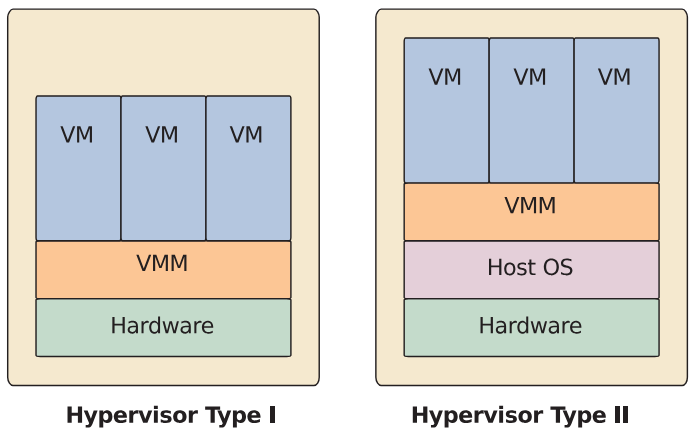
\includegraphics[scale=0.5]{virtualization-hypervisor1.png}
	\caption{انواع هایپروایزر \cite{virtualization1}}
	\label{fig: hypervisors types}
\end{figure}

هایپروایزرها به لحاظ انعطاف‌پذیری و امکان پیکربندی متنوع، قابلیت‌های قدرتمندی را برای مدیریت سرورهای مجازی فراهم می‌کنند. آنها می‌توانند به طور خودکار منابع را بین ماشین‌های مجازی تخصیص دهند و امکاناتی مانند تکثیر\footnote{\lr{Replication}} و بازیابی فاجعه\footnote{\lr{Disaster Recovery}} را ارائه دهند.

ماشین مجازی\footnote{\lr{Virtual Machine (VM)}} واحدی از منابع مجازی است که شبیه‌سازی یک سرور فیزیکی را انجام می‌دهد. هر \lr{VM} می‌تواند سیستم‌عامل خود را داشته باشد و مستقل از دیگر \lr{VM}‌ها عمل کند. این امر به کاربران اجازه می‌دهد که برنامه‌های متعدد را بدون تداخل با یکدیگر اجرا کنند. \lr{VM}‌ها از منابع سخت‌افزاری تخصیص داده شده توسط هایپروایزر استفاده می‌کنند و می‌توانند به راحتی از یک سرور فیزیکی به دیگری با استفاده از تکنیک‌هایی نظیر \lr{Snapshot} منتقل شوند. 

استفاده از تکنولوژی مجازی‌سازی نقش بسیار مهمی در فرآیندهای \lr{DevOps} دارد. با امکان ایجاد و حذف سریع ماشین‌های مجازی، مجازی‌سازی به تیم‌های توسعه این امکان را می‌دهد که به سرعت محیط‌های نرم‌افزاری مورد نیاز خود را راه‌اندازی و پس از اتمام کار، آن‌ها را به راحتی حذف کنند، که این امر منجر به صرفه‌جویی در هزینه‌ها و منابع می‌شود. علاوه بر این، مجازی‌سازی ریسک‌های مرتبط با استقرار نهایی در محیط تولید را کاهش داده و با ایجاد محیط‌های شبیه‌سازی شده برای آزمایش‌های پیش از استقرار، اطمینان حاصل می‌کند که نرم‌افزار قبل از راه‌اندازی به درستی کار می‌کند.

\subsection{کانتینرها}

کانتینرها محیط‌هایی هستند که به برنامه‌های نرم‌افزاری امکان می‌دهند تا با تمام وابستگی‌های خود در یک بسته واحد جمع‌آوری شوند. آن‌ها همانند برنامه‌های نرم‌افزاری سنتی که به شما اجازه می‌دهند مستقل از نرم‌افزارهای دیگر و خود سیستم‌عامل کار کنید، نصب نمی‌شوند. مهم‌ترین دغدغه کانتینرها این است که چگونه محیطی فراهم کنند تا نرم‌افزارهایی که در یک محیط پردازشی اجرا می‌شوند با انتقال به محیط دیگر، بدون ایراد و مشکل اجرا شوند. این تکنولوژی از معماری میزبان بهره می‌برد تا از منابع سخت‌افزاری مشترک استفاده کند، اما اجرای برنامه‌ها را در یک محیط ایزوله و مستقل فراهم می‌کند. تمام اجزای ضروری مورد نیاز یک برنامه به‌صورت یک \lr{Image} بسته‌بندی می‌شود. \lr{Image} مربوطه در یک محیط ایزوله اجرا شده و فضای حافظه، \lr{CPU} و فضای ذخیره‌سازی خود را با سیستم‌عامل به اشتراک نخواهد گذاشت. این عمل موجب می‌شود که فرآیندهای موجود در کانتینر، قادر به مشاهده سایر فرآیندها در خارج از آن نباشند.
\begin{figure}[t]
	\centering
	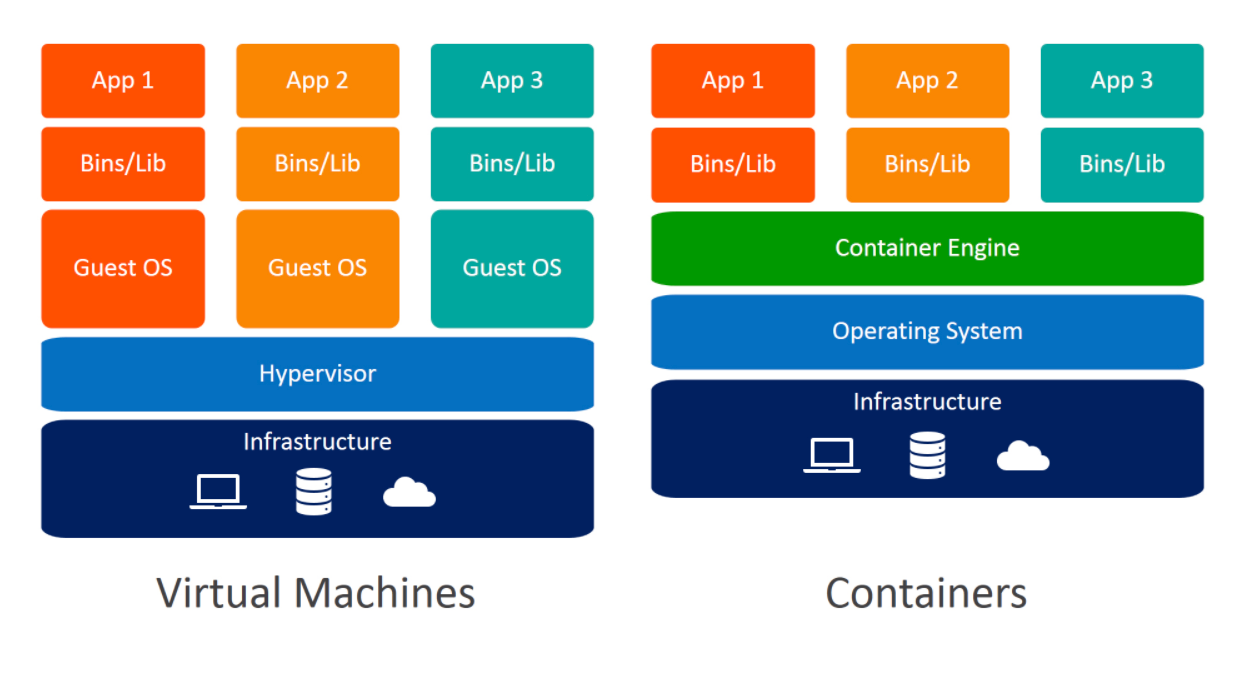
\includegraphics[scale=0.3]{vm-vs-container.png}
	\caption{تفاوت ماشین مجازی و کانتینر}
	\label{fig: vm vs container}
\end{figure}

کانتینرها و ماشین‌های مجازی هر دو ابزارهایی برای ایزوله‌سازی منابع نرم‌افزاری هستند، اما تفاوت‌های اساسی در معماری و کاربرد آن‌ها وجود دارد که در شکل
~\ref{fig: vm vs container}
نشان داده شده است. ماشین‌های مجازی با ایجاد یک لایه انتزاعی کامل بر روی سخت‌افزار فیزیکی کار می‌کنند که به آن‌ها اجازه می‌دهد سیستم‌عامل‌های مستقل را بر روی هر \lr{VM} اجرا کنند. این امر به هر ماشین مجازی امکان می‌دهد منابع سخت‌افزاری را به‌صورت مجزا استفاده کند، اما باعث می‌شود \lr{VM}‌ها نسبت به کانتینرها سنگین‌تر و کم‌استفاده‌تر باشند. در مقابل، کانتینرها به‌جای سیستم‌عامل‌های کامل، تنها برنامه‌ها و وابستگی‌های خود را ایزوله می‌کنند و همگی بر روی هسته سیستم‌عامل میزبان اشتراکی اجرا می‌شوند، که این امر باعث سبک‌تر، سریع‌تر و مقیاس‌پذیرتر شدن کانتینترها نسبت به ماشین‌های مجازی می‌شود. از این رو، کانتینرها برای محیط‌هایی که نیازمند راه‌اندازی سریع و مدیریت منابع مانند میکروسرویس‌ها و برنامه‌های کاربردی مبتنی بر ابر هستند، ایده‌آل می‌باشند \cite{Dockervm}. در کنار مزایای فراوان کانتینترها، برخلاف ماشین‌های مجازی در امنیت و ایزولاسیون داده‌ها محدودیت‌هایی دارند و ممکن است نیازمند ابزارهای پیچیده‌تر برای مدیریت لاگ‌ها و نظارت باشند، که می‌تواند پیاده‌سازی و نگهداری آن‌ها را چالش‌برانگیز سازد.

تکنولوژی کانتینر ریشه در مفهوم چارچوب‌های \lr{Unix} مانند \lr{chroot} دارد که در دهه 1970 معرفی شد. اما، پیشرفت‌های اصلی در این زمینه با ظهور \lr{Docker} در سال 2013 آغاز شد. داکر یک پلتفرم متن‌باز است که استاندارد‌سازی ایجاد، اجرا و مدیریت کانتینرها را فراهم کرد و به‌سرعت به یکی از مهم‌ترین ابزارها در این حوزه تبدیل شد.

اجزای کلیدی مورد استفاده در پیاده‌سازی کانتینرها شامل موارد زیر است \cite{Docker2}:
\begin{itemize}
	\item 
	موتورهای کانتینر\footnote{\lr{Container Engine}}
	\item
	هماهنگ‌سازی کانتینر\footnote{\lr{Container Orchestration}}
\end{itemize}

موتورهای کانتینری مانند \lr{Docker Engine} و \lr{Containerd} ابزارهایی هستند که کانتینرها را ایجاد، اجرا و مدیریت می‌کنند. این موتورها از فناوری‌های موجود در هسته لینوکس مانند \lr{Namespaces} و \lr{Control groups (cgroups)} برای ایزوله‌سازی کانتینرها استفاده می‌کنند و به آن‌ها امکان می‌دهند که فرایندها و منابع سیستمی را به‌صورت مستقل از یکدیگر مدیریت کنند. \lr{Namespaces} بخشی از هسته لینوکس است که امکان جداسازی عناصری مثل شبکه، فرایندها و فضای فایل سیستم را فراهم می‌کند. هر کانتینر در یک \lr{namespace} جداگانه اجرا می‌شود که استقلال آن را نسبت به دیگر برنامه‌ها تضمین می‌کند. \lr{cgroups} نیز به مدیریت استفاده از منابع سخت‌افزاری مانند \lr{CPU} و حافظه توسط فرایندها کمک می‌کند. این فناوری امکان اختصاص دقیق منابع به کانتینرها را می‌دهد و از مصرف بیش‌ازحد منابع توسط یک کانتینر جلوگیری می‌کند.

\lr{Docker Image}
به‌عنوان اساسی‌ترین بخش در اکوسیستم داکر نقش کلیدی در پیاده‌سازی و توزیع برنامه‌های نرم‌افزاری دارد. تصاویر داکر از یک معماری لایه‌ای بهره می‌برند. معماری لایه‌ای این امکان را فراهم می‌کند که تغییرات نسبت به یک تصویر پایه به‌صورت دیفرانسیلی اعمال شود. هر لایه در تصویر داکر، تغییراتی را نسبت به لایه قبلی اضافه می‌کند. این رویکرد باعث می‌شود که بازسازی و به‌روزرسانی تصاویر کانتینری فقط بر روی لایه‌هایی که تغییر کرده‌اند انجام شود، که به نوبه خود باعث کاهش حجم داده‌های موردنیاز برای ذخیره‌سازی و انتقال می‌شود. زمانی که \lr{Dockerfile} نوشته می‌شود، هر دستور (مانند \lr{RUN}, \lr{COPY} و \lr{FROM}) یک لایه جدید در تصویر داکر ایجاد می‌کند. این لایه‌ها به ترتیبی که در داکرفایل آمده‌اند، روی هم اضافه می‌شوند. داکر از یک فایل‌سیستم \lr{Union} استفاده می‌کند که به آن این اجازه را می‌دهد تا لایه‌های مختلف را به‌گونه‌ای ترکیب کند که به نظر یک فایل‌سیستم یکپارچه است \cite{Docker1}. ساختار لایه‌ای تصویر داکر را در شکل 
~\ref{fig: docker image layer}
مشاهده می‌کنید.
\begin{figure}[t]
	\centering
	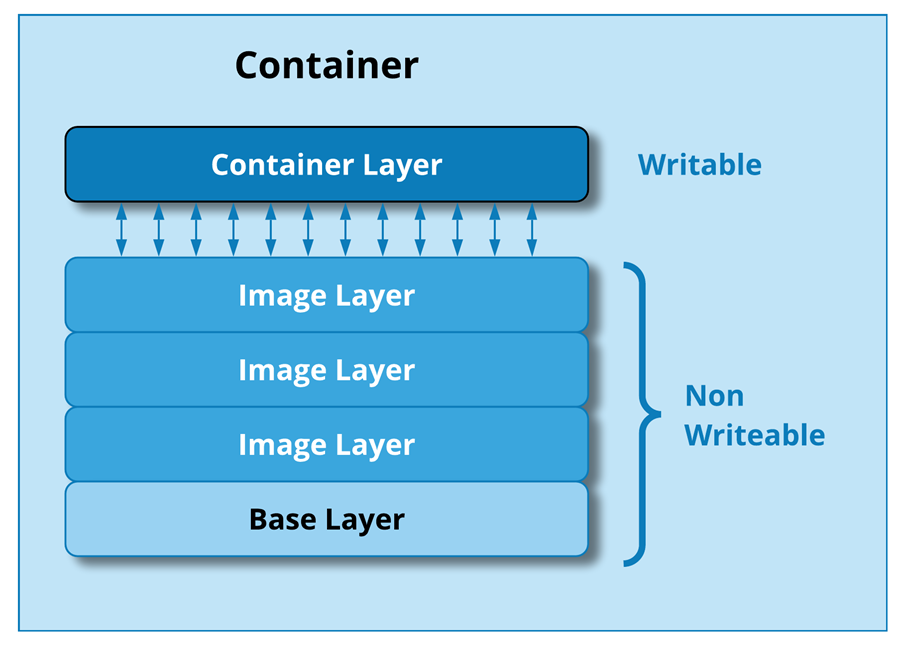
\includegraphics[scale=1]{docker-image-layer1.png}
	\caption{معماری لایه‌ای تصویر داکر}
	\label{fig: docker image layer}
\end{figure}

برای مدیریت و مقیاس‌بندی کانتینرها در محیط‌های تولید، ابزارهای هماهنگ‌سازی مانند \lr{Kubernetes} و \lr{Docker Swarm} کاربرد دارند. این ابزارها به توسعه‌دهندگان این امکان را می‌دهند که خوشه\footnote{\lr{Cluster}}‌های بزرگ کانتینری را مدیریت کنند و برنامه‌ها را با انعطاف‌پذیری و دقت بالا مقیاس‌بندی نمایند.

\subsection{هماهنگ سازی کانتینرها (کوبرنتیز)}

در دنیای توسعه نرم‌افزار، استفاده از معماری‌های مبتنی بر میکروسرویس‌ها و کانتینترها افزایش یافته است که هر دو نیازمند مدیریت دقیق و خودکار سرویس‌ها در محیط‌های تولید هستند. در محیط‌های پویا و با مقیاس بزرگ که دستگاه‌ها و خدمات به طور مکرر تغییر می‌کنند، تقریباً غیرممکن است که با نیروی کار دستی، سرویسی با دسترسی بالا ارائه داد. در چنین شرایطی، ابزارهای هماهنگ‌سازی نقش حیاتی ایفا می‌کنند. آن‌ها به خودکارسازی مدیریت کانتینترها، مدیریت شبکه و نظارت بر سلامت سیستم کمک می‌کنند. بدون هماهنگ‌سازی تیم‌های توسعه و عملیات با چالش‌های عدیده‌ای از جمله کنترل ناموفق بر پیکربندی‌ها، مشکلات مربوط به برقراری ارتباط بین سرویس‌ها، دشواری‌های مربوط به مقیاس‌پذیری و برقراری تعادل بار مواجه می‌شوند. در میان ابزارهای هماهنگ‌سازی \lr{Kubernetes} به‌عنوان یکی از پیشروان بازار شناخته می‌شود که امکان مدیریت خودکار مجموعه‌های بزرگی از کانتینترها را فراهم می‌آورد. کوبرنتیز یک پلتفرم هماهنگ‌سازی کانتینتر است که فرایند زمان‌بندی\footnote{\lr{Scheduling}}، خودکارسازی استقرار، مدیریت و مقیاس‌گذاری اپلیکیشن‌های کانتینتری را تسهیل می‌کند.

\subsubsection{معماری کوبرنتیز}
یک سیستم کوبرنتیز با تمام اجزای آن را یک خوشه\footnote{\lr{Cluster}} می‌گویند. هر خوشه شامل یک یا چند گره\footnote{\lr{Node}} است که می‌توانند فیزیکی\footnote{\lr{Bare-metal}} یا مجازی باشند. این گره‌ها به دو دسته اصلی یا همان سطح کنترل\footnote{\lr{Control plane}} و کاری\footnote{\lr{Worker}} تقسیم می‌شوند.
گره اصلی به‌عنوان مغز متفکر کوبرنتیز عمل می‌کند و وظایف مدیریتی خوشه را بر عهده دارد. این گره شامل مولفه‌های اصلی زیر است:

\begin{figure}[t]
	\centering
	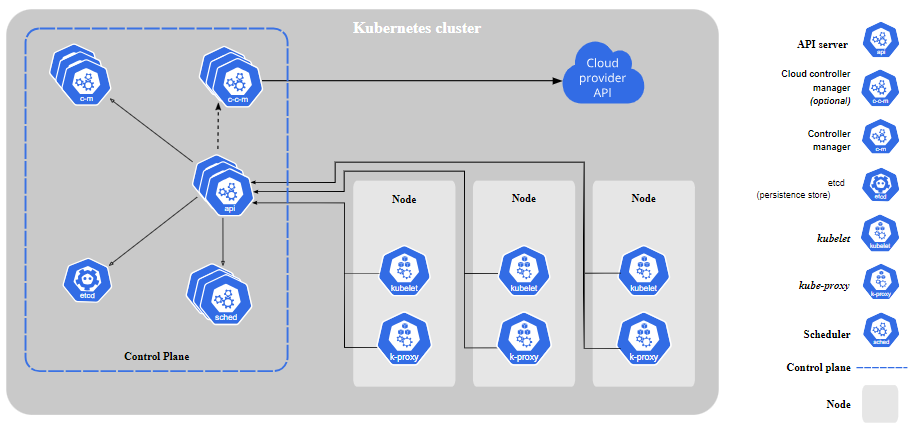
\includegraphics[scale=0.6]{components-of-kubernetes.png}
	\caption{مولفه‌های یک خوشه کوبرنتیز}
	\label{fig: components of kuber}
\end{figure}

\begin{itemize}
	\item 
	\lr{API Server}: 
	نقطه اصلی دریافت فرمان‌های کوبرنتیز به‌صورت \lr{REST}\footnote{\lr{Representational State Transfer}} است و آن را پردازش می‌کند. این سرور مسئول اعتبارسنجی درخواست‌ها و اجرای آن‌ها بر روی خوشه است. همچنین، این مولفه به‌عنوان بخشی از مولفه‌های دیگر گره اصلی عمل می‌کند تا اطمینان حاصل شود که دستورات به درستی اجرا می‌شوند.
	\item 
	\lr{Scheduler}: 
	مولفه‌ای است که تصمیم می‌گیرد کدام پادها بر روی کدام گره‌های کاری قرار گیرند. این فرایند بر اساس منابع موجود و الزامات مشخص شده برای پادها صورت می‌گیرد. علاوه بر این، به‌طور مداوم وضعیت خوشه را رصد می‌کند تا بهترین تصمیم‌ها را برای مکان‌یابی پادها بگیرد.
	\item 
	\lr{Controller Managers}:
	مجموعه‌ای از فرآیندهایی است که حلقه‌های نظارتی را اجرا می‌کنند. این کنترل‌کننده‌ها وضعیت خوشه را با حالت مطلوب مطابقت می‌دهند. به‌عنوان مثال، اگر یک پاد از کار افتاده باشد، یک کنترل‌کننده وظیفه دارد تا یک پاد جدید را برای جایگزینی ایجاد کند.
	\item 
	\lr{etcd}: 
	یک پایگاه داده توزیع شده است که تمام داده‌های مهم از جمله وضعیت خوشه در هر لحظه، پیکربندی خوشه، اطلاعات مربوط به هر گره و کانتینترهای درون آن را در خود ذخیره می‌کند. 
\end{itemize}

گره‌های کاری نیز پادهای اپلیکیشن‌های کاربر را بر عهده دارند. این گره‌ها شامل مولفه‌های زیر هستند:
\begin{itemize}
	\item 
	\lr{Kubelet}:
	این مولفه وظیفه مدیریت سلامت پادها را بر عهده دارد. علاوه بر این اطمینان حاصل می‌کند که کانتینترها در پادها بر اساس تنظیمات مشخص شده اجرا شوند و با \lr{API Server} ارتباط برقرار کند تا وضعیت را به‌روز رسانی کند.
	\item
	\lr{Kube-proxy}: 
	وظیفه مدیریت ترافیک شبکه درون خوشه را بر عهده دارد. این مولفه ارتباطات شبکه بین کانتینترها را تسهیل می‌کند و از قوانین \lr{IPTables} برای مسیریابی ترافیک استفاده می‌کند.
\end{itemize}

\subsubsection{پاد و \lr{Deployment}}
پاد در کوبرنتیز کوچک‌ترین واحد قابل استقرار و مدیریت است که شامل یک یا چند کانتینتر می‌شود. این کانتینترها به‌طور معمول از یک فضای ذخیره‌سازی و شبکه مشترک استفاده می‌کنند و می‌توانند به‌راحتی با یکدیگر ارتباط برقرار کنند. هر پاد دارای یک آدرس \lr{IP} یکتا است که امکان ارتباط مستقیم بین کانتینترها را فراهم می‌کند. پادها به‌صورت موقت طراحی شده‌اند و ممکن است به دلایل مختلفی مانند بروزرسانی یا مشکلات سیستمی حذف و بازسازی شوند. معمولاً پادها برای اجرای یک برنامه خاص (مانند یک سرور وب) استفاده می‌شوند، اما در مواردی که نیاز به همکاری نزدیک کانتینترها باشد، می‌توانند چندین کانتینتر مرتبط را نیز شامل شوند.

\lr{Deployment} 
در کوبرنتیز ابزاری قدرتمند برای مدیریت و مقیاس‌پذیری برنامه‌ها است. این ابزار به کاربران امکان می‌دهد تا مجموعه‌ای از پادها را تعریف و به‌سادگی مدیریت کنند. کاربران می‌توانند نسخه‌های جدید برنامه‌ها را منتشر کرده، مقیاس آن‌ها را تنظیم و در صورت بروز مشکل به نسخه‌های قبلی بازگردند. همچنین، به‌طور خودکار وضعیت پادها را مانیتور می‌کند و در صورت نیاز، آن‌ها را مجدداً راه‌اندازی می‌کند تا اطمینان حاصل شود که همیشه تعداد مشخصی از پادها در حال اجرا هستند. این ویژگی‌ها آن را به گزینه‌ای مناسب برای مدیریت برنامه‌های پایدار و قابل‌اعتماد در محیط‌های تولیدی تبدیل می‌کند.

\subsubsection{مدیریت داده}
در کوبرنتیز، \lr{Volume} مکانیزمی است که به پادها اجازه می‌دهد به داده‌های پایدار دسترسی داشته باشند. هر \lr{Volume} به یک پاد متصل شده حتی با پایان یافتن پاد، داده‌ها می‌توانند حفظ شوند. انواع مختلفی از \lr{Volume}ها وجود دارد که عبارتند از:
\begin{itemize}
	\item 
	\lr{emptyDir}:
	این نوع \lr{Volume} زمانی که پاد ایجاد می‌شود، ساخته شده و هنگام حذف پاد، از بین می‌رود. برای ذخیره‌سازی موقتی مناسب است.
	\item
	\lr{hostPath}: 
	به فایل یا دایرکتوری روی گره میزبان اشاره می‌کند. این گزینه به مواردی که به دسترسی مستقیم به منابع میزبان نیاز دارند، کمک می‌کند.
	\item 
	\lr{PersistentVolume (PV), PersistentVolumeClaim (PVC)}:
	از اجزای اصلی برای مدیریت داده‌های پایدار هستند. \lr{PV} به‌عنوان منبع ذخیره‌سازی مستقل ایجاد می‌شود و شامل ویژگی‌هایی مانند ظرفیت و حالت‌های دسترسی است. \lr{PVC} یک درخواست از طرف کاربر برای استفاده از \lr{PV} است. \lr{PVC}ها به‌طور خودکار به \lr{PV}های موجود متصل می‌شوند که شرایط مورد نیاز را برآورده کنند.
	\item 
	\lr{configMap}:
	برای وارد کردن داده‌های پیکربندی به‌عنوان فایل‌ها در پادها استفاده می‌شود.
	\item 
	\lr{secret}:
	برای ذخیره داده‌های حساس مانند رمزهای عبور به‌صورت رمزگذاری شده و دسترسی به آن‌ها به‌عنوان فایل در پادها.
\end{itemize}
























